\documentclass{article}

\usepackage[utf8]{inputenc}
\usepackage{amsthm}
\usepackage{amssymb}
\usepackage{mathtools}
\usepackage{graphicx}
\usepackage{mdframed}
\usepackage{float}
\usepackage[top=0.75in, bottom=0.75in, left=0.75in, right=0.75in]{geometry}
\usepackage{gauss}

\usepackage{array}
\allowdisplaybreaks

\makeatletter
\newcounter{elimination@steps}
\newcolumntype{R}[1]{>{\raggedleft\arraybackslash$}p{#1}<{$}}
\def\elimination@num@rights{}
\def\elimination@num@variables{}
\def\elimination@col@width{}
\newenvironment{elimination}[4][0]
{
    \setcounter{elimination@steps}{0}
    \def\elimination@num@rights{#1}
    \def\elimination@num@variables{#2}
    \def\elimination@col@width{#3}
    \renewcommand{\arraystretch}{#4}
    \start@align\@ne\st@rredtrue\m@ne
}
{
    \endalign
    \ignorespacesafterend
}
\newcommand{\step}[2]
{
    \ifnum\value{elimination@steps}>0\sim\quad\fi
    \left[
        \ifnum\elimination@num@rights>0
            \begin{array}
            {@{}*{\elimination@num@variables}{R{\elimination@col@width}}
            |@{}*{\elimination@num@rights}{R{\elimination@col@width}}}
        \else
            \begin{array}
            {@{}*{\elimination@num@variables}{R{\elimination@col@width}}}
        \fi
            #1
        \end{array}
    \right]
    & 
    \begin{array}{l}
        #2
    \end{array}
    \addtocounter{elimination@steps}{1}
}
\makeatother

\DeclarePairedDelimiter{\abs}{\lvert}{\rvert}
\DeclarePairedDelimiter{\norm}{\lvert \lvert}{\rvert \rvert}

\newtheoremstyle{break}% name
  {}%         Space above, empty = `usual value'
  {}%         Space below
  {\itshape}% Body font
  {}%         Indent amount (empty = no indent, \parindent = para indent)
  {\bfseries}% Thm head font
  {.}%        Punctuation after thm head
  {\newline}% Space after thm head: \newline = linebreak
  {}%         Thm head spec

\newtheorem{Def}{Definition}[section]

\theoremstyle{break}

\newtheorem{innerEx}{Exempel}[section]
\newtheorem{sats}{Sats}[section]
\newtheorem{Rem}{Anmärkning}[]

\newenvironment{Ex}
{\begin{mdframed} \begin{innerEx} \vspace{3pt}}
{\vspace{3pt} \end{innerEx} \end{mdframed}}  

\newenvironment{bevis}
{\begin{mdframed} \begin{proof} \vspace{3pt}}
{\vspace{3pt} \end{proof} \end{mdframed}}

\title{
	 Linjär Algebra\\
	 Föreläsning 8
    \author{Erik Sjöström}
}
\begin{document}
\maketitle
\section{Linjära avbildningar (forts)} % (fold)
\label{sec:linj_ra_avbildningar_}
Kom ihåg:
\begin{align*}
&&f:\mathbb{R}^n \rightarrow \mathbb{R}^m
&&&\mbox{ och }
&&&&f(\vec{x}) = \mathbf{A} \cdot \vec{x}
\end{align*}
Låt:
\begin{align*}
&f:\mathbb{R}^n \rightarrow \mathbb{R}^m
&&g:\mathbb{R}^n \rightarrow \mathbb{R}^m
\end{align*}
vara två linjära avbildningar och:
\begin{align*}
&f(\vec{x}) = \mathbf{A} \cdot \vec{x}
&&g(\vec{x}) = \mathbf{B} \cdot \vec{x}
\end{align*}
Då gäller för $f+g$ att:
\[
    f(\vec{x}) + g(\vec{x}) = \mathbf{A} \cdot \vec{x} + \mathbf{B} \cdot \vec{x} = (\mathbf{A} + \mathbf{B}) \cdot \vec{x}
\]
$(f+g)$ är också linjär avbildning med standardmatris $(\mathbf{A}+\mathbf{B})$\\
För $c \cdot f$ där $c \in \mathbb{R}$ gäller:
\[
    c \cdot f(\vec{x}) = c \cdot \mathbf{A} \cdot \vec{x} = (c \cdot \mathbf{A}) \cdot \vec{x}
\]
dvs $(c \cdot f)$ är också en linjär avbildning med standardmatris $(c \cdot \mathbf{A})$\\
Låt 
\begin{align*}
&f:\mathbb{R}^n \rightarrow \mathbb{R}^p
&&f:\mathbb{R}^p \rightarrow \mathbb{R}^m
\end{align*}
vara två linjära avbildningar med standardmatriser, $\mathbf{A}_{p \times n}$ repektive $\mathbf{B}_{m \times p}$\\
Då gäller för den sammansatta avbildningen:
\[
    g(f(\vec{x})) = g(\mathbf{A} \cdot \vec{x}) = \mathbf{B}(\mathbf{A} \cdot \vec{x}) = (\mathbf{B} \cdot \mathbf{A}) \cdot \vec{x}
\]
dvs en linjär avbildning med standardmatris $(\mathbf{B} \cdot \mathbf{A})$
\begin{Rem}
    Den sammansatta funktionen $g(f(\vec{x}))$ skrivs vanligtvis som $g \circ f(\vec{x})$
\end{Rem}
\newpage
\begin{Ex}
	\textbf{Rotation}
	\begin{center}
		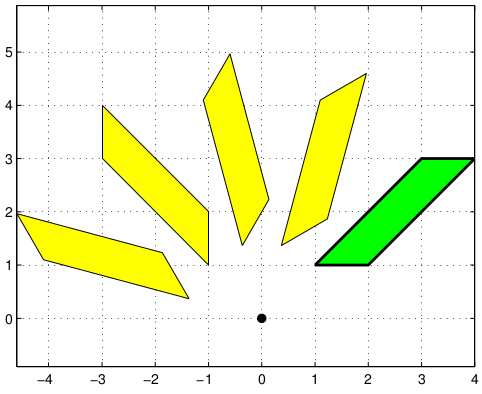
\includegraphics[scale=0.5]{F7.png}
	\end{center}
    Grönt område beskrivs av hörnen:
    \begin{align*}
		&\vec{x}_1 = \begin{bmatrix} 1\\1 \end{bmatrix}
	    &&&\vec{x}_2 = \begin{bmatrix} 3\\3 \end{bmatrix}
	    &&&&\vec{x}_3 = \begin{bmatrix} 4\\3 \end{bmatrix}
	    &&&&&\vec{x}_4 = \begin{bmatrix} 2\\1 \end{bmatrix}
    \end{align*}
    $f:\mathbb{R}^2 \rightarrow \mathbb{R}^2$ och $f(\vec{x}) = \mathbf{A} \cdot \vec{x}$ där:
    \[
        \mathbf{A} = \begin{bmatrix} cos(\pi/6)&-sin(\pi/6)\\sin(\pi/6)&cos(\pi/6)\end{bmatrix} 
    \]
    Hörnpunkten i 1:a gula 4-hörningen ges av:
    \begin{align*}
    &\vec{y}_1 = \mathbf{A} \cdot \vec{x}_1,
    &&\vec{y}_2 = \mathbf{A} \cdot \vec{x}_2,
    &&&\vec{y}_3 = \mathbf{A} \cdot \vec{x}_3,
    &&&&\vec{y}_4 = \mathbf{A} \cdot \vec{x}_4
    \end{align*}
    Hörnpunkterna för den andra gula 4-hörningen fås genom att rotera bilderna $\vec{y}_1 \cdots \vec{y}_4$
    \begin{align*}
    &A \cdot \vec{y}_1 = \mathbf{A} \cdot (\mathbf{A} \cdot \vec{x_1}),
    &&A \cdot \vec{y}_2 = \mathbf{A} \cdot (\mathbf{A} \cdot \vec{x_2}),
    &&&A \cdot \vec{y}_3 = \mathbf{A} \cdot (\mathbf{A} \cdot \vec{x_3}),
    &&&&A \cdot \vec{y}_4 = \mathbf{A} \cdot (\mathbf{A} \cdot \vec{x_4})
    \end{align*}
    Vi har alltså en sammansatt avbildning $f(f(\vec{x}))$
\end{Ex}

\begin{Ex}
    Bestäm standardmatrisen för den linjära avbildninger $\mathbb{R}^2 \rightarrow \mathbb{R}^2$ som först roterar $(\pi/6)$ radianer moturs och sedan projiceras ortogonal på x-axeln.
    \[
        \mbox{Rotationen: } f(\vec{x}) = \mathbf{A} \cdot \vec{x} = \begin{bmatrix} \cos(\pi/6)&-\sin(\pi/6)\\\sin(\pi/6)&\cos(\pi/6) \end{bmatrix} \cdot \vec{x}
    \]
    \[
        \mbox{Projektionen: } g(\vec{x}) = \mathbf{B} \cdot \vec{x} = \begin{bmatrix} g(\vec{e}_x)&g(\vec{e}_y) \end{bmatrix} \cdot \vec{x} = \overbrace{\begin{bmatrix} \vec{e}_x&\o \end{bmatrix}}^\text{projektion på x} \cdot \vec{x}= \begin{bmatrix} 1&0\\0&0 \end{bmatrix} \cdot \vec{x}
    \]
    Så om vi först roterar och sedan projicerar får vi:
    \[
        g(f(\vec{x})) = \begin{bmatrix} 1&0\\0&0 \end{bmatrix} \cdot \begin{bmatrix} \cos(\pi/6)&-\sin(\pi/6)\\\sin(\pi/6)&\cos(\pi/6) \end{bmatrix} \cdot \vec{x} = \begin{bmatrix} \cos(\pi/6)&-\sin(\pi/6)\\0&0 \end{bmatrix} \cdot \vec{x}
    \]
    Om vi istället först projicerar och sedan roterar får vi:
    \[
        f(g(\vec{x})) = \begin{bmatrix} \cos(\pi/6)&-\sin(\pi/6)\\\sin(\pi/6)&\cos(\pi/6) \end{bmatrix} \cdot \begin{bmatrix} 1&0\\0&0 \end{bmatrix} \cdot \vec{x} = \begin{bmatrix} \cos(\pi/6)&0\\\sin(\pi/6)&0 \end{bmatrix} \cdot \vec{x}
    \]
    Vi kan alltså se att ordningen spelar roll:
    \[
        f(g(\vec{x})) \neq g(f(\vec{x}))
    \]
    De har alltså olika sandardmatriser, detta kommer från räknereglerna för matriser:
    \[
        \mathbf{A} \cdot \mathbf{B} \neq \mathbf{B} \cdot \mathbf{A}
    \]
\end{Ex}
% section linj_ra_avbildningar_ (end)
\section{Invertering} % (fold)
\label{sec:invertering}
En avbildning:
\[
    f:\mathbb{R}^n \rightarrow \mathbb{R}^n
\]
kallas inverterbar om det finns en linjär avbildning:
\[
    g:\mathbb{R}^n \rightarrow \mathbb{R}^n
\]
sådan att:
\[
    \begin{cases}
		g(f(\vec{x})) = \vec{x}\\
		&\forall \vec{x} \in \mathbb{R}^n \\
		f(g(\vec{x})) = \vec{x}
	\end{cases}
\]
$g$ kallas då för inversen till $f$ och betecknas $f^{-1}$\\
Om $f$ har standardmatrisen $\mathbf{A}$ ($f(\vec{x} = \mathbf{A} \cdot \vec{x}$) så är \textit{f} inverterbar om \textbf{A} är inverterbar, då har $g=f^{-1}$ standardmatrisen $\mathbf{A}^{-1}$ ($g(\vec{x}) = \mathbf{A}^{-1} \cdot \vec{x}$)

\begin{Ex}
    Låt $f:\mathbb{R}^2 \rightarrow \mathbb{R}^2$ vara rotationen motsols med vinkeln $\theta$
    \[
        \mathbf{A} = \begin{bmatrix} \cos(\theta)&-\sin(\theta)\\\sin(\theta)&\cos(\theta) \end{bmatrix}
    \]
    Inversen:
    \[
        \mathbf{A}^{-1} = \frac{1}{d} \begin{bmatrix} \cos(\theta)&\sin(\theta)\\-\sin(\theta)&\cos(\theta) \end{bmatrix}
    \]
    där d är determinanten av \textbf{A}:
    \[
        d = det(\mathbf{A}) = \cos(\theta) \cdot \cos(\theta) - (-\sin(\theta) \cdot \sin(\theta)) = \cos^2(\theta) + sin^2(\theta) = 1
    \]
    Genom att uttrycka:
    \[
        \begin{cases}
        	\cos(-\theta) = \cos(\theta)\\
        	\sin(-\theta) = -\sin(\theta)
        \end{cases}
    \]
    får vi:
    \[
        \mathbf{A}^{-1} = \begin{bmatrix} \cos(-\theta)&-\sin(-\theta)\\\sin(-\theta)&\cos(-\theta) \end{bmatrix}
    \]
    dvs: En rotation $-\theta$ moturs\\
    dvs: Rotation $\theta$ medurs\\
    En rotation moturs med vinkeln $\theta$ följt av en rotation medurs med vinkeln $\theta$ gör att vi är tillbaka där vi startade.
    dvs: \textbf{A} och $\mathbf{A}^{-1}$ är inverser.
\end{Ex}
% section invertering (end)
\section{Translation} % (fold)
\label{sec:translation}
En translation:
\begin{align*}
&t_b:\vec{x} + \vec{t} &&t=\begin{bmatrix} t_1\\t_2 \end{bmatrix}\\
&t_b(\vec{x}) = \vec{x} + \vec{t}
\end{align*}
är alltså själva förflyttningen.
\begin{Ex}
\textbf{Translation}
	\begin{center}
		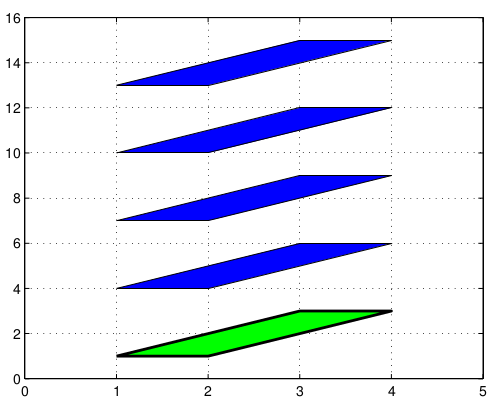
\includegraphics[scale=0.5]{F7plan.png}
	\end{center}
    Grönt område beskrivs av hörnen:
    \begin{align*}
    &&\vec{x}_1 = \begin{bmatrix} 1\\1 \end{bmatrix}
    &&&\vec{x}_2 = \begin{bmatrix} 2\\1 \end{bmatrix}
    &&&&\vec{x}_3 = \begin{bmatrix} 3\\3 \end{bmatrix}
    &&&&&\vec{x}_4 = \begin{bmatrix} 4\\3 \end{bmatrix}
    \end{align*}
    Hörnen translateras genom att addera $\vec{t} = \begin{bmatrix} 0\\3 \end{bmatrix}$\\
    dvs: $\vec{x}_1$ har translateras till:
    \[
        \begin{bmatrix} 1\\1 \end{bmatrix} + \begin{bmatrix} 0\\3 \end{bmatrix} = \begin{bmatrix} 1\\4 \end{bmatrix}
    \]
    och $\vec{x}_2$ till:
    \[
        \begin{bmatrix} 2\\1 \end{bmatrix} + \begin{bmatrix} 0\\3 \end{bmatrix} = \begin{bmatrix} 2\\4 \end{bmatrix}
    \]
    osv.
\end{Ex}

% section translation (end)

\section{Affin avbildning} % (fold)
\label{sec:affin_avbildning}
En affin avbildning är sammansattning av en linjär avbildning och en translation $t_b$\\
Låt:
\begin{align*}
&g:\mathbb{R}^2 \rightarrow \mathbb{R}^2\\
&g(\vec{x}) = \mathbf{A} \cdot \vec{x}
\end{align*}
En  affin avbildning:
\[
    t_b(g(\vec{x})) = t_b(\mathbf{A} \cdot \vec{x}) = \mathbf{A} \cdot \vec{x} \cdot \vec{t}
\]
\begin{Ex}
    Man kan alltid göra om en affin avbildning till en linjär avbildning:\\
    Låt:
    \[
         f(\vec{x}) = \mathbf{A} \cdot \vec{x} + \vec{t}
    \]
    vara en affin avbildning i planet, med:
    \begin{align*}
    &\mathbf{A} = \begin{bmatrix} a_{11}&a_{12}\\a_{21}&a_{22} \end{bmatrix}
    &&\vec{x} = \begin{bmatrix} x\\y \end{bmatrix}
    &&&\vec{t} = \begin{bmatrix} t_1\\t_2 \end{bmatrix}
    \end{align*}
    Vi får då:
    \begin{align*}
        f(\begin{bmatrix} x\\y \end{bmatrix}) &= \begin{bmatrix} a_{11}&a_{12}\\a_{21}&a_{22} \end{bmatrix} \begin{bmatrix} x\\y \end{bmatrix} + \begin{bmatrix} t_1\\t_2 \end{bmatrix} \\
        &= \begin{bmatrix} a_{11} \cdot x + a_{12} \cdot y\\a_{21} \cdot x + a_{22} \cdot y \end{bmatrix} + \begin{bmatrix} t_1\\t_2 \end{bmatrix} \\
        &= \begin{bmatrix} a_{11} \cdot x + a_{12} \cdot y + t_1\\a_{21} \cdot x + a_{22} \cdot y + t_2\end{bmatrix}
    \end{align*}
    Vi bildar en linjär avbildning $g:\mathbb{R}^3 \rightarrow \mathbb{R}^3$ med standardamtris:
    \[
        \mathbf{A}_1 = \begin{bmatrix} a_{11}&a_{12}&t_1\\a_{21}&a_{22}&t_2\\0&0&1 \end{bmatrix}
    \]
    den är linjär så vi kan skriva:
    \[
        g(\begin{bmatrix} x\\y\\1 \end{bmatrix}) = \mathbf{A}_1 \cdot \begin{bmatrix} x\\y\\1 \end{bmatrix} = \begin{bmatrix} a_{11}&a_{12}&t_1\\a_{21}&a_{22}&t_2\\0&0&1 \end{bmatrix} \begin{bmatrix} x\\y\\1 \end{bmatrix} = \begin{bmatrix} a_{11}x + a_{12}y + t_1\\a_{21}x + a_{22}y + t_2\\1 \end{bmatrix}
    \]
    Dvs: representera den affina avbildningen i planet med en linjär avbildning i rummet.
\end{Ex}

% section affin_avbildning (end)

\end{document}